\subsection{Architettura Complessiva} \label{sec:overall-architecture}
L'architettura di Scala Party è pensata per essere completamente modulare, scollegando 
il quanto più possibile il gioco alla base dai minigiochi o dalla forma della 
plancia. Questa struttura consente di espandere più facilmente l'applicazione in futuro e 
aumenta la manutenibilità del codice, oltre a permettere un migliore suddivisione dei 
compiti.

Per questo, l'architettura si divide nei seguenti componenti principali:
\begin{itemize}
    \item \textbf{PartyController}: è il componente principale del gioco, che gestisce le
    regole e le interazioni tra i vari componenti. Funziona come collante tra la
    logica di gioco e l'interazione dell'utente.
    \item \textbf{PartyView}: è la parte dell'applicazione che si occupa di mostrare
    l'interfaccia utente e di gestire le interazioni con il giocatore.
    \item \textbf{PartyGame}: racchiude la logica di gioco generale, come la gestione
    del turno dei giocatori, il lancio dei dadi, il conteggio dei punti e la gestione 
    delle condizioni di vittoria.
    \item \textbf{PartyBoard}: rappresenta la plancia di gioco e gestisce la disposizione
    delle monadi, le caselle piolo e il movimento dei giocatori.
    \item \textbf{PartyPlayer}: rappresenta il giocatore utente e contiene le informazioni
    relative al suo stato, come i pioli e le monadi possedute, oltre alla posizione sulla
    plancia.
    \item \textbf{PartyBotPlayer}: rappresenta il giocatore avversario gestito dal computer, 
    che simula le azioni di un giocatore umano cercando di comportarsi allo stesso modo.
    \item \textbf{Minigame}: viene creato all'inizio di un minigioco la cui logica viene
    scelta casualmente tra quelle disponibili. Gestisce le regole specifiche del
    minigioco, come il punteggio, le condizioni di vittoria e l'interazione del giocatore.
\end{itemize}

In figura \ref{fig:sequence-diagram} è mostrato un diagramma di sequenza che illustra
come i vari componenti interagiscono tra loro durante il gioco. Si può notare come, 
nella maggior parte dei casi, sia il \texttt{PartyController} a iniziare le interazioni
e a coordinare le azioni tra gli altri componenti. Il diagramma è suddiviso in sezioni
che rappresentano le fasi di gioco principali definite nelle regole:
\begin{itemize}
    \item \textbf{Game Start}: è il primo momento del gioco, in cui il giocatore inizia
    una nuoca partita e il \texttt{PartyController} segnala al \texttt{PartyGame} di 
    inizializzare una nuova plancia con i due giocatori al suo interno.
    \item \textbf{Update View}: è un momento particolare in quanto verrà ripetuto molteplici
    volte durante tutto il corso del gioco, sebbene sia mostrato solo la prima volta.
    Il \texttt{PartyController} chiede al \texttt{PartyGame} le informazioni necessarie
    per aggiornare il gioco, che verranno poi mandate a \texttt{PartyView} affinché possa
    mostrarle correttamente all'utente.
    \item \textbf{Dice Roll}: è il momento in cui il giocatore può lanciare i dadi e assume
    un diverso significato a seconda della fase del gioco. È il giocatore a decidere il 
    momento in cui lanciare i dadi, ma il \texttt{PartyGame} è responsabile della generazione
    del numero casuale e della gestione del turno.
    \item \textbf{Player Move}: è il momento in cui il giocatore viene spostato sulla
    plancia in base al risultato del lancio dei dadi. Il \texttt{PartyController} chiede
    al \texttt{PartyGame} di spostare il giocatore, ma prima che ciò sia possibile 
    deve essere richiesto all'utente di scegliere la direzione da prendere fra quelle 
    disponibili. 
    \item \textbf{Minigame}: è il momento in cui viene avviato un nuovo minigioco del quale
    vengono mostrate le regole al giocatore.
\end{itemize}

\begin{figure}[ht!]
    \centering
    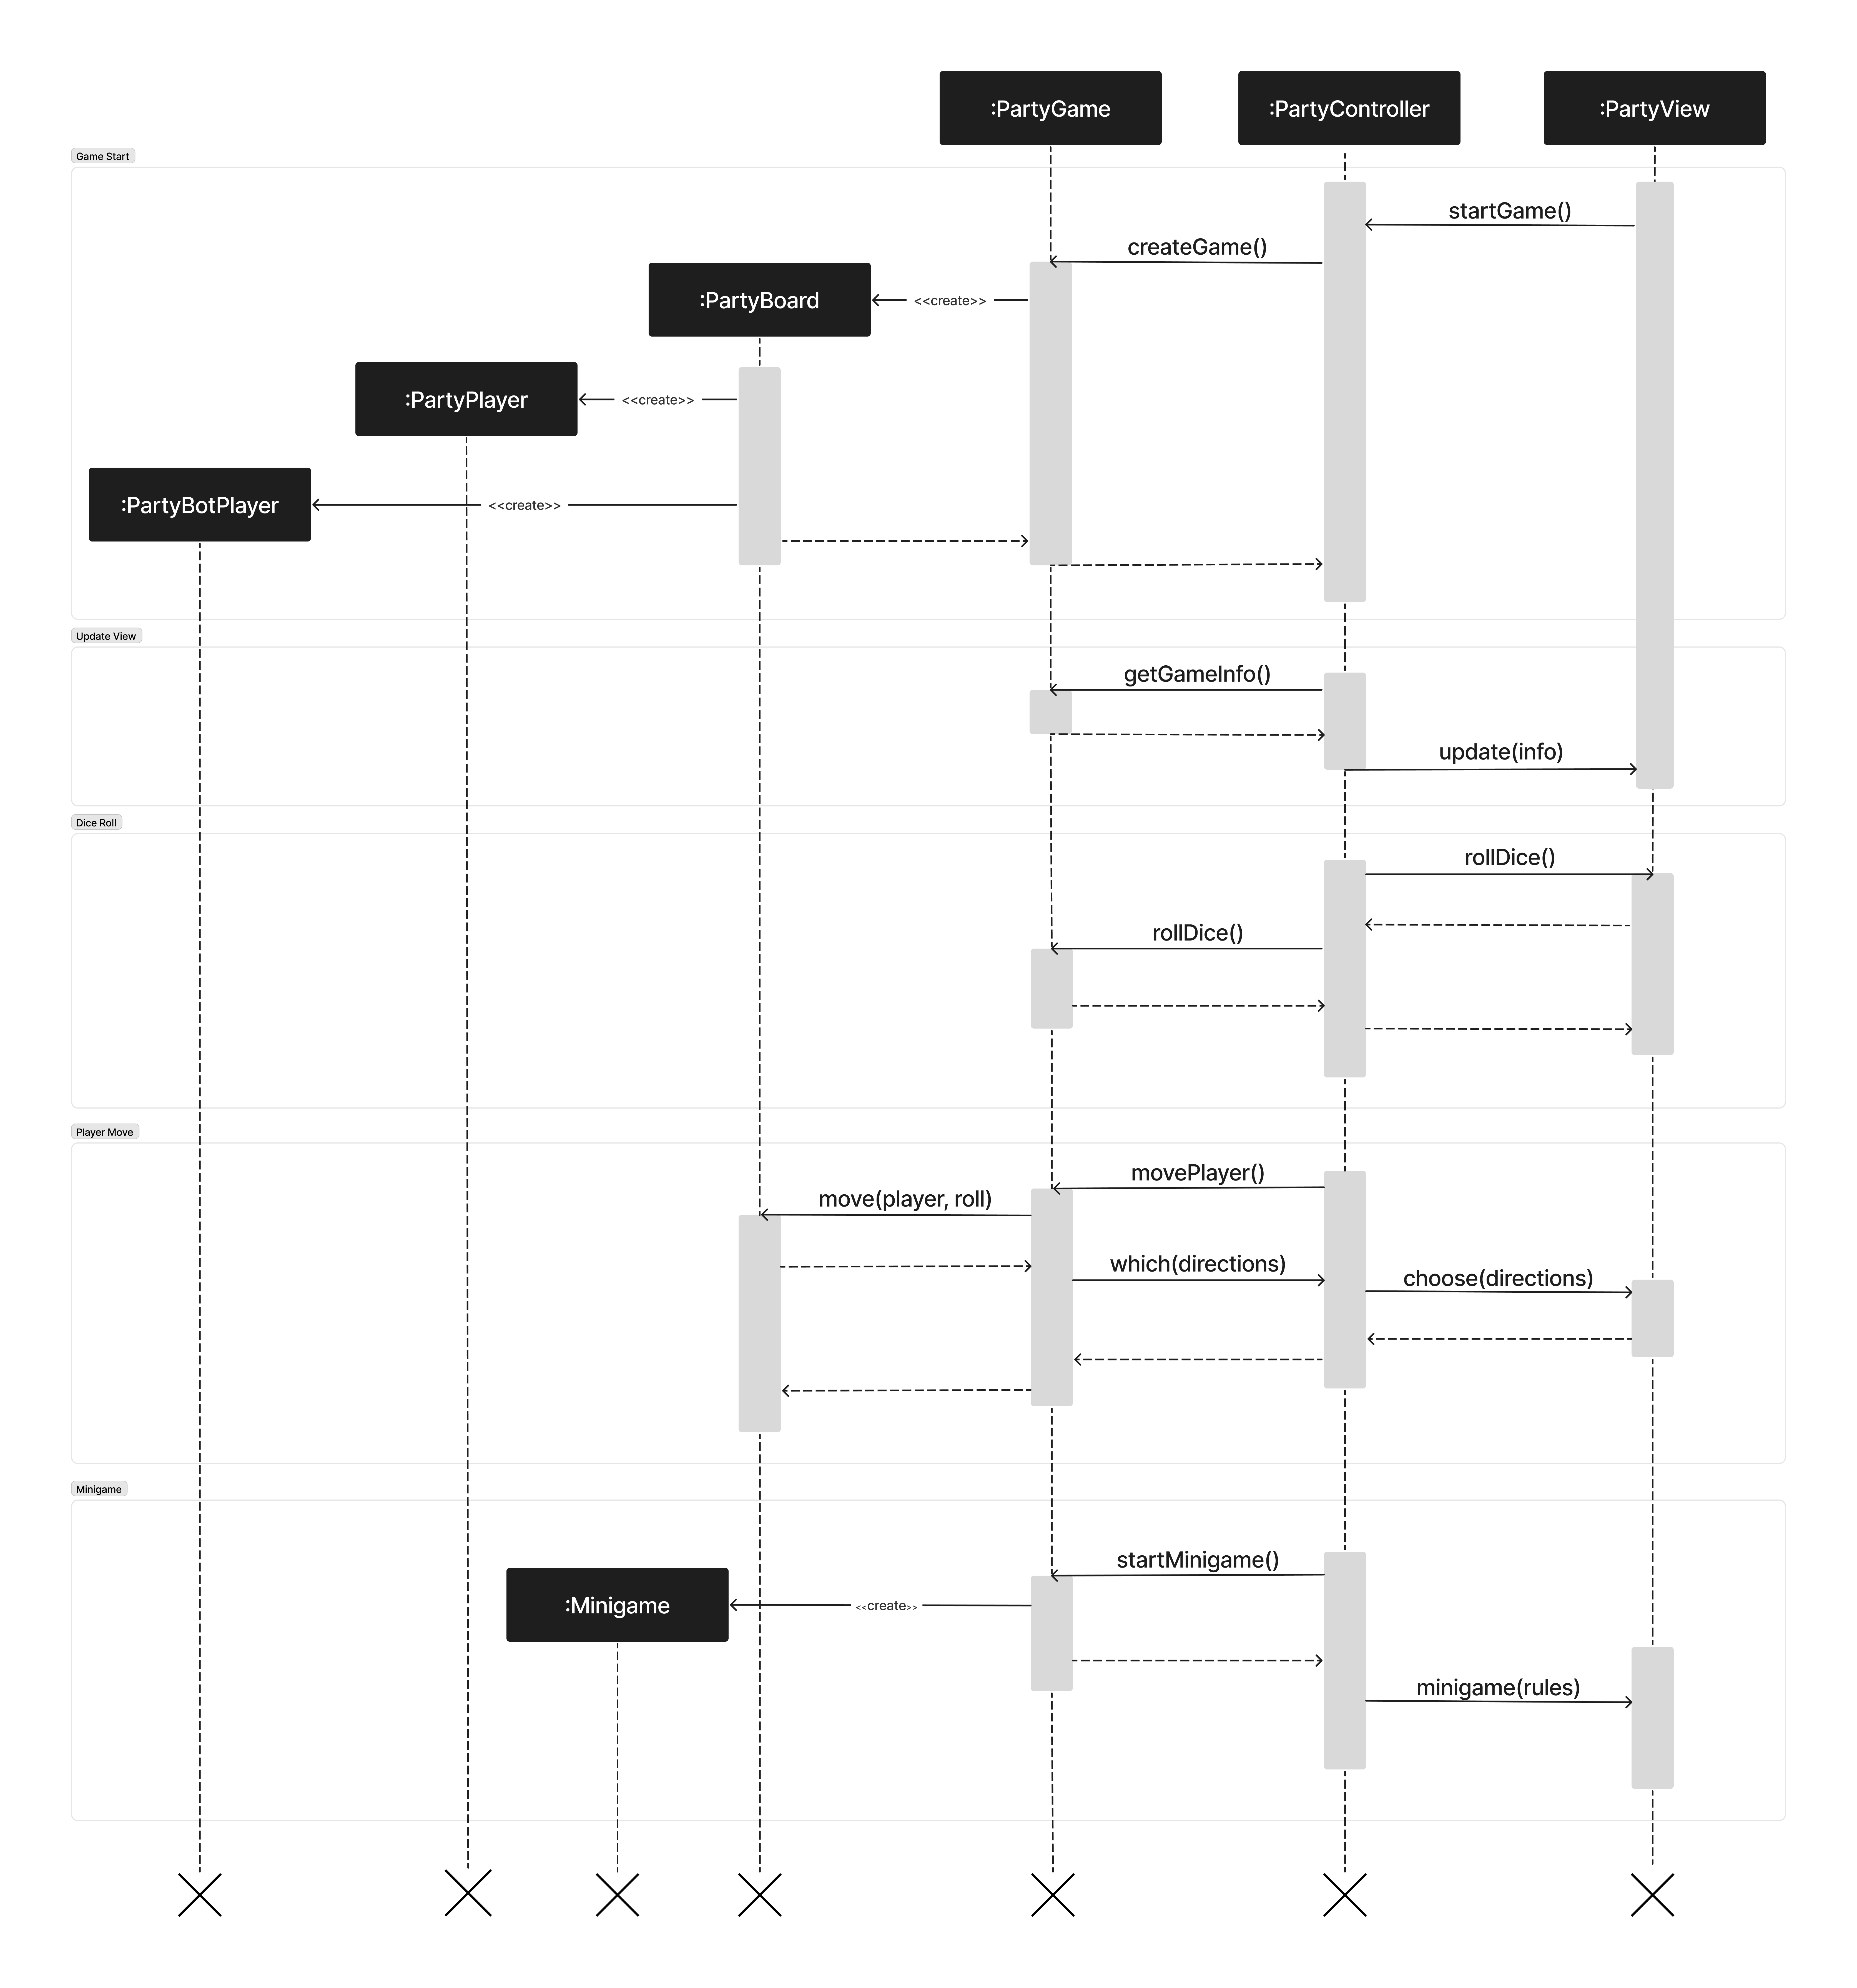
\includegraphics[width=1\textwidth]{figures/sequence-diagram.png}
    \caption{Diagramma di Sequenza dell'architettura}
    \label{fig:sequence-diagram}
\end{figure}